\section{Spracovávané Dáta}

Budeme spracovávať štatistické dáta pacientov, ktorý užívali dva rôzne lieky (nikdy nie naraz) proti primárnej chorobe. Máme k dispozícii dáta o vzorke 10 000 pacietov.


K dispozícii máme, aký liek bol podávaný pacientovi a aký účinok to malo na jeho primárne ochorenie. Ďalej máme k dispozícii základné fyzické proporcie pacienta ako: vek, index telesnej hmotnosti a priemerný krvný tlak. Je nám známa taktiež anamnéza pacienta (výskyt sekundárnych chorôb pred a po liečbe a iná nešpecifikovaná medikácia).

\subsection{Vekové spektrum}

Máme k dispozícii dáta pacientov so širokým vekovým spektrom v rozsahu od 22 až do 70 rokov. Dáta v grafickej podobe môžme vidieť na Obr. \ref{fig:hist-vek}. Histogram udáva absolútny počet pacientov v jednotlivých vekových kategóriach. V tabuľke \ref{tab:vek} je rozdelenie pacientov do vekových podskupín. V analýze budeme pracovať práve s danými podskupinami.

\begin{figure}[h!]
	\centering
  		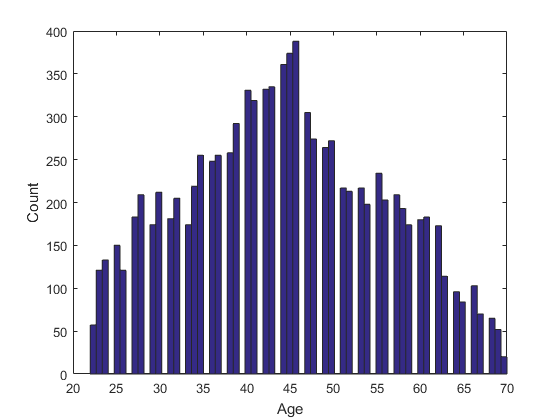
\includegraphics[width=0.9\textwidth]{ages.png}
  	\caption{Histogram Vekov}
  	\label{fig:hist-vek}
\end{figure}

\begin{table}[h!]
\centering
\label{vek}
\begin{tabular}{c|cccccc}
\hline
\textbf{Vek}             & \textless 24 & 25-34 & 35-44 & 45-54 & 55-64 & 65\textless \\ \hline
\textbf{Počet Pacientov} & 311 & 1828  & 2986  & 2722  & 1759  & 394 \\ \hline
\end{tabular}
\caption{Vek pacientov}
\label{tab:vek}
\end{table}

\subsection{BMI Spektrum}

BMI (ang. Body Mass Index) je index telesnej hmotnosti. Je to pomer medzi aktuálnou váhou a výškou\textsuperscript 2.